\documentclass{article}
\usepackage{arxiv}

\usepackage[utf8]{inputenc}
\usepackage[english, russian]{babel}
\usepackage[T1]{fontenc}
\usepackage{url}
\usepackage{booktabs}
\usepackage{amsfonts}
\usepackage{nicefrac}
\usepackage{microtype}
\usepackage{lipsum}
\usepackage{lmodern}
\usepackage{graphicx}
\usepackage{natbib}
\usepackage{doi}

\usepackage[figurename=Figure,tablename=Table]{caption}

\title{Iterative Improvement of a Topic Model with User Feedback}

\author{ Alex Gorbulev \\
	\texttt{gorbulev.ai@phystech.edu} \\
	\And
	Vasiliy Alexeev \\
	\texttt{vasiliy.alekseyev@phystech.edu} \\
	\And
    Konstantin Vorontsov \\
    \texttt{vokov@forecsys.ru} \\
}
\date{}

\renewcommand{\undertitle}{A Preprint}
\renewcommand{\shorttitle}{Iterative Improvement of a Topic Model with User Feedback}

%%% does not show
%%% DeclareMathOperator*{\norm}{norm}

%%% Add PDF metadata to help others organize their library
%%% Once the PDF is generated, you can check the metadata with
%%% $ pdfinfo template.pdf
%%% \hypersetup{
%%% pdftitle={A template for the arxiv style},
%%% pdfsubject={q-bio.NC, q-bio.QM},
%%% pdfauthor={David S.~Hippocampus, Elias D.~Striatum},
%%% pdfkeywords={First keyword, Second keyword, More},
%%% }

\begin{document}
\maketitle

\begin{abstract}
    We introduce the method of topic modeling using user feedback. The user marks a topic as relevant, irrelevant, or "garbage". The main problem is to improve the base model preserving relevant topics. The number of "garbage" \ topics should decrease. We provide the solution using topic modeling algorithms and regularizers for sparsing and decorrelation. We run the experiment on Lenta.ru news dataset.
\end{abstract}

\keywords{Topic Modeling \and ARTM \and Natural language processing}

\section{Introduction}
Topic modeling is the actually developing \citep{10031921} method of text analysis, which is used in sociological studies \citep{DIMAGGIO2013570}.
Topic model estimates a probability of belonging to one of the topics.
Topic modeling was used in studies of Croatian news during COVID-19 pandemic \citep{pandemic2021} and Lithuanian media representation of climate change \citep{climate2021}.

However, learning a topic model is an ill-posed problem with an infinite set of solutions \citep{bigartm}.
To bound the number of solutions, we add regularization penalty terms.
For example, decolleration improves topic coherence \citep{artm2}, sparsing regularization increases the number of zero elements of matrices.

During the study period, only a part of topics could be relevant.
At the same time, irrelevant topics, which duplicate relevant topics, and "garbage" \ topics, which are not related to the research, could contain relevant documents. To improve the quality of the research, we should reveal as more relevant texts as possible.

Our goal is to build an interpretable renewable topic model using user feedback.
The user markup consists of topic distribution by category: relevant, irrelevant and "garbage" \ topics. The improvement of the model preserves previously found relevant topics and determines new relevant topics in place of "garbage" \ topics.

To solve the problem, we use additive regularization of topic models (ARTM). Open source libraries \texttt{BigARTM} and \texttt{TopicNet} \citep{bulatov-etal-2020-topicnet} implement the methods of ARTM and include regularizers for decorrelation and smoothing. In ARTM, we optimize the topic model by a sum of criteria \citep{artm}. We use Lenta.ru news dataset. The dataset consists of $16449$ articles in Russian language from May, 2008 to August, 2008.

\section{Problem Statement}

Let $D$ denote a set of texts and $W$ denote a set of all terms from these texts.
Each term can represent a single word or a key phrase \citep{artm2}.
Each document $d \in D$ is a sequence of $n_d$ terms $\left( w_1, \dots, w_{n_d} \right)$ from the set $W$ \citep{artm}.
The set of topics $T$ is finite.
Text collection $D$ is considered to be a sample drawn independently from a discrete distribution $p(w, d, t)$ over a finite space $W \times D \times T$ \citep{artm2}.
According to the law of total probability and the assumption of conditional independence \citep{bigartm}:
 \begin{equation}
      p(w \mid d) = \sum \limits_{t \in T} p(w \mid t, d) p(t \mid d) = \sum \limits_{t \in T} p (w \mid t) p (t \mid d) = \sum \limits_{t \in T} \varphi_{wt} \theta_{td}
 \end{equation}
The problem of topic modeling is to find parameters $\varphi_{wt}$ and $\theta_{td}$ by text collection D that approximate frequency estimates for the conditional probabilities of $\widehat{p} (w \mid d)$.
In most cases, the number of topics $|T|$ is much smaller than the vocabulary size $|W|$ and the collection size $|D|$. This problem is equivalent to finding an low-rank stochastic matrix decomposition \citep{artm2}
\begin{equation}
     F \approx \Phi \Theta
\end{equation}
where $F = {(\widehat{p}_{wd})}_{|W| \times |D|}$ is the matrix of term frequencies in documents, $\Phi = {(\varphi_{wt})}_{|W| \times |T|}$ is the matrix of terms of the topics, $\Theta = {(\theta_{td})}_{|T| \times |D|}$ is the matrix of topics of the documents.

Let $T^i$ denote a set of topics on the iteration $i \in \mathbb{N}$,  $T_+^i \subset T^i$ denote a subset of relevant topics, $T_0^i \subset T^i$ denote a subset of irrelevant topics, $T_-^i \subset T^i$ denote a subset of "garbage" \ topics, $M_i$ denote a model on the iteration $i$, where $T^i = T_+^i \sqcup T_0^i \sqcup T_-^i$.
The iterative improvement of the model $M_i$ is the building of the model  $M_{i + 1}$, where the set of topics $T_{i + 1}$ satisfies the following requirements:

$$T_+^i \subset T_+^{i + 1}, \ \left| T_-^{i + 1} \right| \leq \left| T_-^{i + 1} \right|$$

\section{Method}

We assume to learn the new model $M_{i + 1}$ using additive regularization of topic models (ARTM) by following steps:

\begin{enumerate}
    \item Set the alternative value of a random seed;
    \item Fix the columns of the matrix $\Phi$ corresponding to relevant topics $T_+^i$ by sparsing regularizer \citep{SukVor19}
    \begin{equation}
        R (\Phi, \Theta) = \beta_0 \sum \limits_{t \in T_+} \sum \limits_{w \in W} \beta_{wt} \widetilde{\varphi}_{wt} \ln \varphi_{wt}
    \end{equation}
    The matrix $\widetilde{\Phi}$ corresponds to the matrix of the model $M_i$. To fix the topics, we should use this regularizer with sufficiently large coefficient. During the experiment, we use the topic fixing regularizer with a coefficient $\beta_0 = {10}^9$.
    \item Use the regularizer of decorrelation to reveal new relevant topics:
    \begin{equation}
        R(\Phi) = -\tau \sum \limits_{t \in T_- \cup T_0} \sum \limits_{s \in T_-} \sum \limits_{w \in W} \varphi_{wt} \widetilde{\varphi}_{ws} \to \max
    \end{equation}
    \begin{equation}
        R(\Phi) = -\tau \sum \limits_{t \in T_- \cup T_0 \\ s \in T_-} \left\langle \varphi_t, \widetilde{\varphi}_s \right\rangle \to \max
    \end{equation}
    \begin{equation}
        R(\Phi) = -\tau \sum \limits_{t \in T_- \cup T_0} \left\langle \varphi_t, \sum \limits_{s \in T_-} \widetilde{\varphi}_s \right\rangle \to \max
    \end{equation}
    \begin{equation}
        \frac{\partial R}{\partial \varphi_{wt}} = -\tau [t \in T_- \cup T_0] \sum \limits_{s \in T_-} \widetilde{\varphi}_{ws}
    \end{equation}
    \begin{equation}
        \varphi_{wt} = {norm}_{w \in W} \left(n_{wt} - \tau \varphi_{wt} [t \in T_- \cup T_0] \sum \limits_{s \in T_-} \widetilde{\varphi}_{ws}\right)
    \end{equation}
\end{enumerate}

As external criterion, we use the number of relevant topics $|T_+|$ and the number of "garbage" \ topics $|T_-|$.
The more $|T_+|$ and less $|T_-|$, the better.

We assume to use the following metrics as internal criteria:

\begin{enumerate}
    \item Perplexity \citep{bigartm}
    \begin{equation}
        \mathcal{P}_m (D; p) = \exp \left( - \frac{1}{n_m} \sum \limits_{d \in D} \sum \limits_{w \in W^m} n_{dw} \ln p (w \mid d) \right)
    \end{equation}
    \item Sparsity of the matrix $\Phi$
    \item Average topic contrast \citep{bigartm}, where we define the contrast of the topic as
    \begin{equation}
        {con}_t = \frac{1}{|W_t|} \sum \limits_{w \in W_t} p(t \mid w)
    \end{equation}
    \begin{equation}
        W_t = \{ w \in W \mid \varphi_{wt} > \frac{1}{|W|} \}
    \end{equation}
\end{enumerate}

\section{Experiment}

The code of the \href{https://github.com/intsystems/2023-Project-131/blob/master/code/Experiment_Tuning_Last.ipynb}{experiment} is written in Python. We use the open source libraries BigARTM and TopicNet.

\subsection{Dataset Description}

To learn topic models, we use \href{https://disk.yandex.ru/d/DAdhmVB2eFkdBQ}{Lenta.ru news dataset}.
The dataset contains $16 449$ news articles in Russian from May 1, 2008 to August 31, 2008.
Each article belongs to one of the $11$ categories:

\begin{enumerate}
    \item <<Бывший СССР>> (English: The Former USSR)
    \item <<Дом>> (English: Home)
    \item <<Из жизни>> (English: From the Life)
    \item <<Интернет и СМИ>> (English: The Internet and the Media)
    \item <<Культура>> (English: Culture)
    \item <<Мир>> (English: World)
    \item <<Наука и техника>> (English: Science and Tech)
    \item <<Россия>> (English: Russia)
    \item <<Силовые структуры>> (English: Security Forces)
    \item <<Спорт>> (English: Sport)
    \item <<Экономика>> (English: Economics)
\end{enumerate}

The user could mark up different news articles from one category as belonging to relevant topic or "garbage" \ topic. To provide more precise clusterization, we assume to set the number of topics $|T|$ at $50$.

\subsection{Preprocessing}

We split the title and the text of each article into tokens.
Each token represents a single word.
Next, we use the morph analyzer \texttt{pymorphy2} \citep{pymorphy2} to lemmatize tokens.
At the same time, we exclude stop-words from the tokens set.
We create bigrams from two consequent lemmatized tokens.
The next step is to choose top-$10 000$ bigrams by pointwise mutual information (PMI).
We represent each document as a sequence of the selected bigrams.
To work with TopicNet, we convert our token data to Vowpal Wabbit format.

The total elapsed time is $11$ minutes $14$ seconds.

\subsection{Base Model}

As the base model $M_0$, we use the topic model without regularizers corresponding to $|T|$ specific topics. The model $M_0$ has regularizers for sparsing the columns of the matrices $\Phi$ and $\Theta$ related to a single background topic. The corresponding coefficients are equal to $0$.
We use two modalities:
\begin{enumerate}
    \item Lemmatized tokens (\texttt{@lemmatized}), the coefficient is $1.0$;
    \item Bigrams (\texttt{@bigram}), the coefficient is $0.8$.
\end{enumerate}
The value of the parameter \texttt{seed} is equal to $21$.
We learn the model $M_0$ by $50$ iterations.

\subsection{Creating the New Model}

Let we know the user markup based on the topic model $M_{i - 1}$ and the parameters of $M_{i - 1}$.
We create the model $M_i$ by following steps::
\begin{enumerate}
    \item We increase the value of the parameter \texttt{seed} by $21$;
    \item Using regularizer $(3)$, fix the topics from $T_+^{i - 1}$;
    \item Create the decorrelation regularizer $(4)$ for topics from $T_0^{i - 1}$ and $T_-^{i - 1}$;
    \item Save another parameters of the model the same.
\end{enumerate}
Inexistience of the determined solution \citep{bigartm} is one of the disadvantages of topic modeling. Topic models are dependent on the randomness. To reduce dependence, we vary the value of the parameter \texttt{seed}. Each value is unique for each version of the model.

\subsection{Results}

After the training of the model $M_0$, the user identified $5$ relevant topics:

\begin{enumerate}
    \item $12$ (Dmitry Medvedev, international relationships)
    \item $21$ (the conflict in Georgia, August 2008)
    \item $29$ (the politics of Ukraine)
    \item $30$ (2008 United States presidential election)
    \item $35$ (Putin as Prime Minister of Russia)
\end{enumerate}

The user identified the topic $31$ as irrelevant for duplication the topic $21$.
Next, we created the model $M_1$. The regularizer $(3)$ preserved previously found relevant topics. Moreover, the user identified $2$ new relevant topics:
\begin{enumerate}
    \item $14$ (sanctions against Iran)
    \item $15$ (the politics of Zimbabwe, elections)
\end{enumerate}
Next, we created the model $M_2$. The sparsing regularizer preserved each topic from $T_+^1$ as relevant. The user identified the topic $46$ (Hague Tribunal) as new relevant topic.
After training the new model $M_3$, the user markup remained the same.

\begin{table}[]
    \centering
    \begin{tabular}{c|c|c|c|}
        Model & $|T_+|$ & $|T_0|$ & $|T_-|$ \\
        \hline
        $M_0$ & $5$ & $1$ & $44$ \\
        $M_1$ & $7$ & $1$ & $42$ \\
        $M_2$ & $8$ & $1$ & $41$ \\
        $M_3$ & $8$ & $1$ & $41$
    \end{tabular}
    \caption[Table 1]{User markup data}
    \label{tab:my_label}
\end{table}

\newpage

By each modality, the models $M_1$ и $M_2$ have bigger perplexity than the model $M_0$.
In most cases, topic models without regularizers have less perplexity than topic models with regularizers  \citep{artm2}.
At the same time, after $50$ iterations the perplexity of the model $M_3$ is similar to the perplexity of the model $M_0$.

\begin{figure}[h]
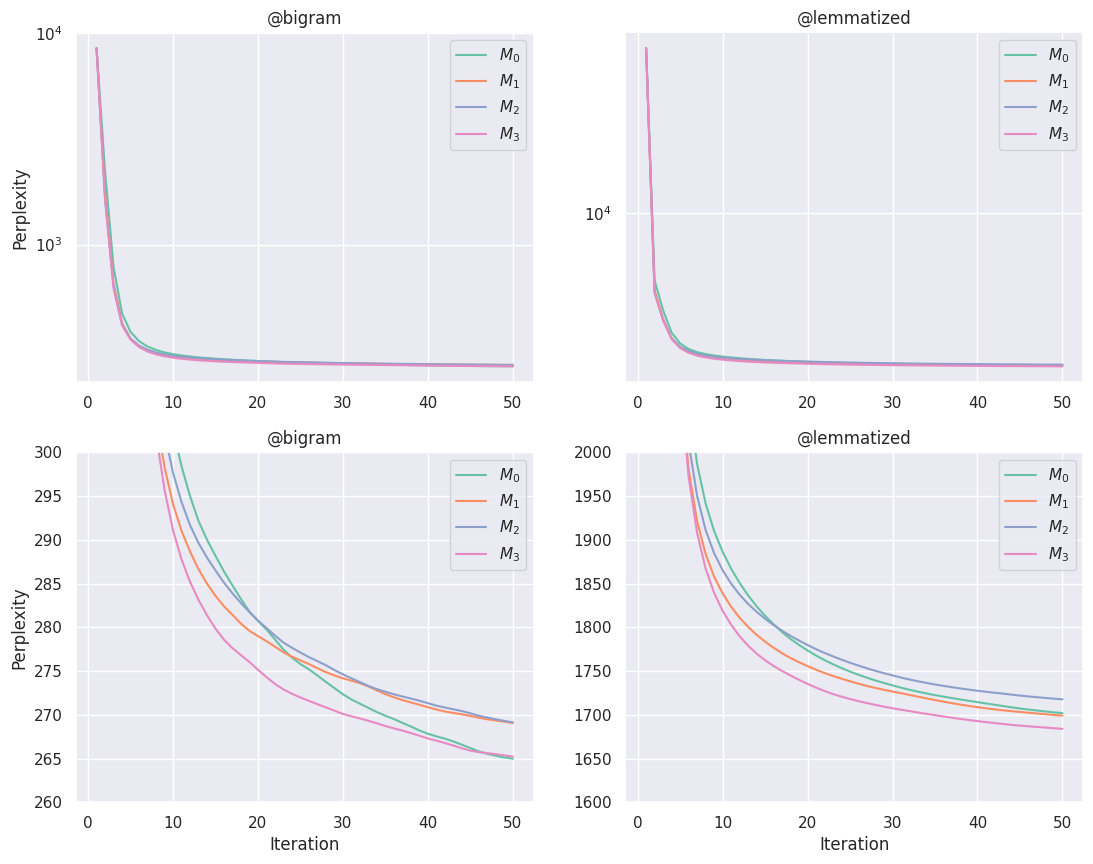
\includegraphics[width=8cm]{figures/perplexity_v3.png}
\centering
\caption{Perplexity}
\end{figure}

The sparsity of the matrix $\Phi$ varies slightly from model to the model.

\begin{figure}[h]
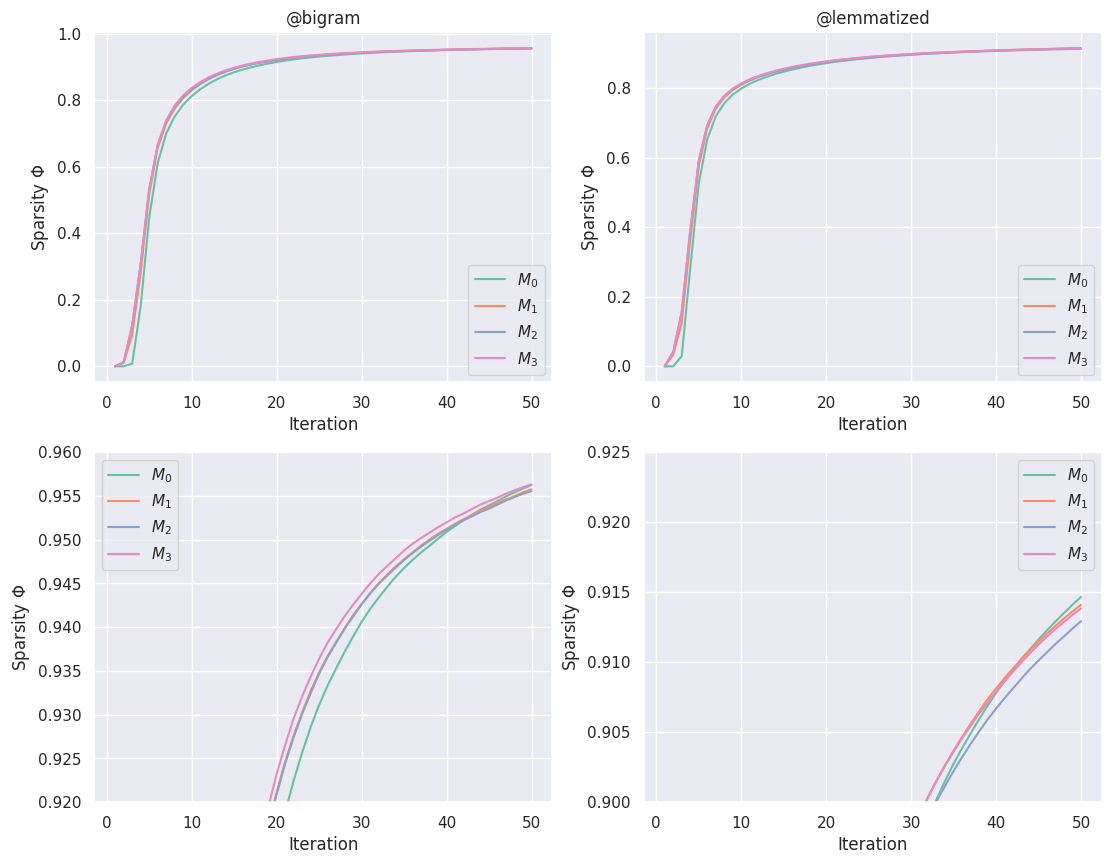
\includegraphics[width=8cm]{figures/sparsity_v3.png}
\centering
\caption{Sparsity of the $\Phi$}
\end{figure}

By average topic contrast, the models $M_0$ and $M_3$ show the similar results.
By lemmatized tokens modality, the model $M_0$ has the biggest average topic contrast.
At the same time, the differencies are quite small.

\begin{figure}[h]
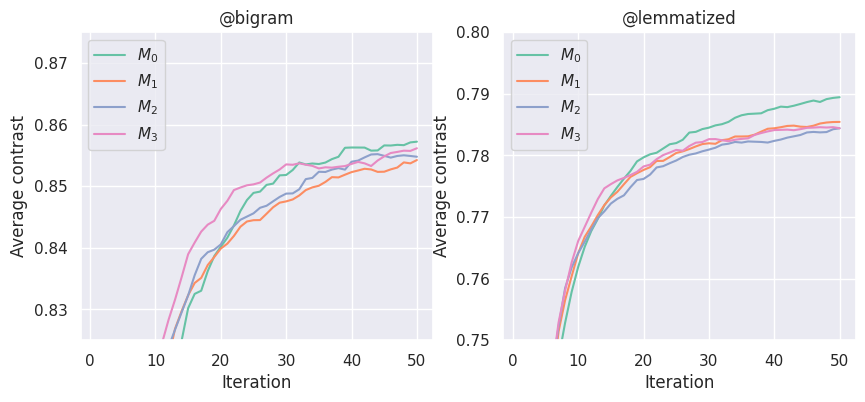
\includegraphics[width=8cm]
{figures/avg_contrast_v3.png}
\centering
\caption{Average topic contrast}
\end{figure}

\section{Conclusion}

In this paper, we propose the method of the iterative improvement of a topic model. To fix relevant topics, we use sparsing regularizer. To reveal new relevant topics, we use decorrelation regularizer.
In this experiment, the sparsing regularizer preserves relevant topics, and the number of relevant topic increases after using regularizer for the decorrelation.
We plan to conduct new experiments on specialized datasets to test the universality of the proposed method.

\bibliographystyle{plain}
\renewcommand{\refname}{References} 
\bibliography{Gorbulev2023TopicModelsEng}

\end{document}